\section{Services DICOM}

\frame
{
	\frametitle{Services DICOM}
	
	\begin{itemize}
		\item<1-> \'Equivalent des IOD pour les services : DIMSE (DICOM Message Service Element).
		\item<2-> D\'efinir les op\'erations possibles selon les objets.
		\item<3-> Deux cat\'egories d'\'el\'ements :
		\begin{itemize}
			\item<4-> op\'erations (par exemple \emph{store}) ;
			\item<5-> notifications (e.g. \emph{event report}).
		\end{itemize}
		\item<6-> Services diff\'erents selon les objets
		\begin{description}
			\item<7->[Composites] C-STORE, C-FIND, C-MOVE, C-GET, C-ECHO.
			\item<8->[Normalis\'es] N-GET, N-ACTION, N-SET, N-CREATE, N-DELETE, N-EVENT-REPORT.
			\item<9->[Web] QIDO-RS, WADO-RS, WADO-URI, STOW-RS, UPS-RS, CAPABILITIES.
		\end{description}
	\end{itemize}
}

\frame
{
	\frametitle{Services principaux}
	\setbeamertemplate{description item}[align left]
	\begin{description}
		\item<2->[Store] Envoi/stockage d'objets DICOM.
		\item<3->[Storage Commitment] V\'erification de l'archivage d'une image.
		\item<4->[Query/Retrieve]~\\
		\begin{itemize}
			\item<5-> Interrogation par crit\`eres \`a diff\'erents niveaux (e.g. patient, examen, s\'erie, image) :
			\item<6-> R\'ecup\'eration d'images/s\'eries/examens selon ces m\^emes crit\`eres.
		\end{itemize}
		\item<7->[Modality worklist]~\\
		\begin{itemize}
			\item<8-> Interrogation par une modalit\'e du syst\`eme de planification.
			\item<9-> R\'ecup\'eration de la liste des examens pr\'evus.
			\item<10-> Examens document\'es (identito-vigilance) : identification du patient, proc\'edure, prescripteur.
		\end{itemize}
		\item<11->[MPPS] V\'ehiculer les informations sur ce qui est r\'ealis\'e par un syst\`eme.
	\end{description}
}

%\frame
%{
%	\frametitle{Autres services}
%	\setbeamertemplate{description item}[align left]
%	\begin{description}
%		\item<1->[Printing]~\\
%		D\'emod\'e depuis les imprimantes PostScript.
%		\item<2->[Storage commitment]~\\
%		Confirmer qu'un objet est stock\'e de mani\`ere permanente.
%		\item<3->[Modality performed procedure step]~\\
%		Permet de diffuser l'information d'avancement d'un examen.
%		\item<4->[Offline media]~\\
%		D\'etails sur le stockage sur support CD, DVD, etc.
%	\end{description}
%}

\frame
{
	\frametitle{Communication}
	\begin{itemize}
		\item Chaque \'equipement joue un r\^ole d\'ependant du service :
		\begin{description}
			\item<2->[SCU] Service Class User (le client).
			\item<3->[SCP] Service Class Provider (le serveur).
		\end{description}
		\item<4-> Le SCU initie une demande, le SCP, qui fournit le service, r\'epond.
	\end{itemize}
	
	\begin{center}
		\includegraphics<5->[width=.8\linewidth]{./figures/scu-scp.png}
	\end{center}
}

\frame
{
	\frametitle{Changement de r\^ole}
	Un \'equipement peut changer de r\^ole.
	
	Par exemple, une station d'interpr\'etation A peut \^etre :
	\begin{itemize}
		\item<2-> SCU dans un premier temps :
		\begin{enumerate}
			\item<3-> A sollicite un examen au PACS ;
			\item<4-> Le PACS accepte et envoie l'examen \`a A.
		\end{enumerate}
		\item<5-> puis SCP dans un second temps :
		\begin{enumerate}
		\setcounter{enumi}{2}
			\item<6-> B demande l'examen \`a A ;
			\item<7-> A transmet l'examen \`a B.
		\end{enumerate}
	\end{itemize}
	
%	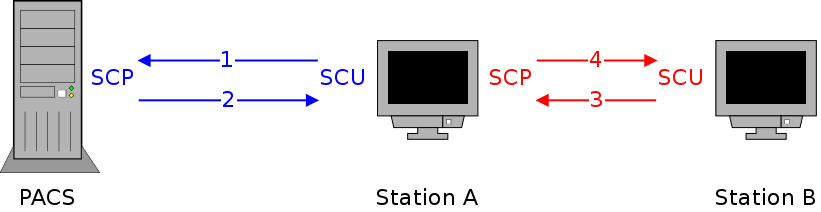
\includegraphics[width=\linewidth]{./figures/roles.png}
	\includegraphics<2>[width=.6\linewidth]{./figures/roles-scu.png}
	\includegraphics<3>[width=.6\linewidth]{./figures/roles-1.png}
	\includegraphics<4>[width=.6\linewidth]{./figures/roles-2.png}
	\includegraphics<5>[width=\linewidth]{./figures/roles-scp.png}
	\includegraphics<6>[width=\linewidth]{./figures/roles-3.png}
	\includegraphics<7>[width=\linewidth]{./figures/roles-4.png}
}
